\documentclass[10pt,a4paper]{article}

% =========================================================================
% Packages
% =========================================================================
\usepackage[utf8]{inputenc}
\usepackage[T1]{fontenc}
\usepackage{lmodern}
\usepackage{geometry}
\usepackage{graphicx}
\graphicspath{{Gambar/}}
\usepackage{amsmath,amssymb}
\usepackage{fancyhdr}
\usepackage{titlesec}
\usepackage{booktabs}
\usepackage{tabularx}
\usepackage{array}
\usepackage{caption}
\usepackage{subcaption}
\usepackage{algorithm}
\usepackage{algpseudocode}
\usepackage{hyperref}
\usepackage{microtype}
\usepackage{url}
\usepackage{cite}
\usepackage{float}
\usepackage{placeins}

% =========================================================================
% Page Geometry & Margins (EPROTIK Standard: A4 Paper, Margins: 2.5 cm all sides)
% =========================================================================
\geometry{
  a4paper,
  top=2.5cm,
  bottom=2.5cm,
  left=2.5cm,
  right=2.5cm,
  headheight=45pt,
  headsep=12pt,
  footskip=22pt
}

% Paragraph settings: Justified, single space
\setlength{\parindent}{0pt}
\setlength{\parskip}{3.5pt}
\linespread{1.0}

% Float Spacing Adjustments
\setlength{\floatsep}{8pt plus 2pt minus 2pt}
\setlength{\textfloatsep}{10pt plus 2pt minus 2pt}
\setlength{\intextsep}{8pt plus 2pt minus 2pt}

% Hyperlink configuration
\hypersetup{
  colorlinks=true,
  linkcolor=blue,
  citecolor=blue,
  urlcolor=blue
}

% =========================================================================
% Header & Footer Settings
% =========================================================================
\pagestyle{fancy}
\fancyhf{}
\fancyhead[L]{\fontsize{9pt}{11pt}\selectfont eProceeding of TIK}
\fancyfoot[R]{\fontsize{9pt}{11pt}\selectfont\thepage}
\renewcommand{\headrulewidth}{0.4pt}
\renewcommand{\footrulewidth}{0pt}

% First page header
\fancypagestyle{firstpage}{
  \fancyhf{}
  \fancyhead[L]{%
    \begin{minipage}[c]{0.78\textwidth}
      {\fontsize{10pt}{12pt}\selectfont\textbf{eProceeding of TIK}}\\[2pt]
      {\fontsize{8.5pt}{10.5pt}\selectfont E-ISSN: 2797-1724, P-ISSN: 3031-1454}\\[1pt]
      {\fontsize{8.5pt}{10.5pt}\selectfont Vol. 7 No. 1 2027 pp. xx--xx}
    \end{minipage}%
  }
  \fancyhead[R]{%
    \begin{minipage}[c]{0.20\textwidth}
      \raggedleft
      \IfFileExists{Gambar/template_eprotik_image5.png}{
\includegraphics[height=1.05cm]{template_eprotik_image5.png}}{%
        \IfFileExists{Gambar/elvira_image5.png}{
\includegraphics[height=1.05cm]{elvira_image5.png}}{}%
      }
    \end{minipage}%
  }
  \fancyfoot[R]{\fontsize{9pt}{11pt}\selectfont\thepage}
  \renewcommand{\headrulewidth}{0.5pt}
  \renewcommand{\footrulewidth}{0pt}
}

% =========================================================================
% Section Headings Formatting
% Level 1: 14pt Bold
% Level 2: 12pt Bold
% Level 3: 10pt Bold
% =========================================================================
\titleformat{\section}
  {\fontsize{14pt}{17pt}\bfseries}{\thesection.}{0.5em}{}
\titlespacing*{\section}{0pt}{12pt}{4pt}

\titleformat{\subsection}
  {\fontsize{12pt}{15pt}\bfseries}{\thesubsection}{0.5em}{}
\titlespacing*{\subsection}{0pt}{9pt}{3pt}

\titleformat{\subsubsection}
  {\fontsize{10pt}{12pt}\bfseries}{\thesubsubsection}{0.5em}{}
\titlespacing*{\subsubsection}{0pt}{6pt}{2pt}

% Caption styles (9 pt / small)
\captionsetup{font={small},labelfont=bf,justification=centering}
\captionsetup[table]{position=top,skip=3pt}
\captionsetup[figure]{position=bottom,skip=4pt}

% =========================================================================
% Document Body
% =========================================================================
\begin{document}
\thispagestyle{firstpage}

% --- Article Title (20pt Bold, Left Aligned) ---
{\fontsize{20pt}{24pt}\bfseries\raggedright Rancang Bangun Aplikasi Point of Sale dengan Fitur Prediksi Penjualan Harian Menggunakan Long Short-Term Memory\par}
\vspace{8pt}

% --- Authors (11pt Regular) ---
{\fontsize{11pt}{13pt}\selectfont Muhammad Kholis$^{1*}$, Zulfan Khairil Simbolon$^{2}$, Azhar$^{3}$\par}
\vspace{4pt}

% --- Affiliations (9pt) ---
{\fontsize{9pt}{11pt}\selectfont
$^{1,2,3}$ Jurusan Teknologi Informasi dan Komputer, Politeknik Negeri Lhokseumawe, Indonesia\par}
\vspace{4pt}

% --- Corresponding Author (9pt) ---
{\fontsize{9pt}{11pt}\selectfont
*Penulis Korespondensi: \href{mailto:parzivalxdd@gmail.com}{parzivalxdd@gmail.com}\par}
\vspace{4pt}

% --- Open Access License (8pt) ---
{\fontsize{8pt}{10pt}\selectfont
This is an open access article under the \href{https://creativecommons.org/licenses/by-sa/4.0/}{CC-BY-SA} license.\par
\vspace{2pt}
\IfFileExists{Gambar/template_eprotik_image1.png}{
\includegraphics[height=0.45cm]{template_eprotik_image1.png}}{%
  \IfFileExists{Gambar/elvira_image1.png}{
\includegraphics[height=0.45cm]{elvira_image1.png}}{}%
}\par}

\vspace{5pt}
\noindent\rule{\textwidth}{0.4pt}
\vspace{3pt}

% --- Abstrak (14pt Heading, 10pt Content) ---
{\fontsize{14pt}{16pt}\bfseries Abstrak\par}
\vspace{4pt}

{\fontsize{10pt}{13pt}\selectfont
Penelitian ini merancang dan membangun aplikasi \textit{Point of Sale} (POS) berbasis \textit{mobile} dengan arsitektur \textit{offline-first} yang dilengkapi fitur prediksi penjualan harian menggunakan metode \textit{Long Short-Term Memory} (LSTM), dengan studi kasus kantin EatsTEDI Universitas Gadjah Mada. Sistem dikembangkan menggunakan \textit{framework} Flutter yang terintegrasi dengan basis data lokal Isar DB dan basis data \textit{cloud} Supabase PostgreSQL, sedangkan modul prediksi dibangun menggunakan Python (TensorFlow dan Flask) dan di-\textit{deploy} sebagai layanan API terpisah. Data penelitian berupa 313 hari aktif transaksi yang dimodelkan sebagai deret waktu univariat dengan target \textit{log-return}. Kinerja model diukur menggunakan metrik MAE, RMSE, dan sMAPE terhadap ambang kelayakan praktis $\text{sMAPE} < 20\%$ melalui dua skenario pengujian. Pada skema satu langkah ke depan (\textit{one-step-ahead}), LSTM Hybrid mencatat MAE Rp667.718,00 dan sMAPE 38,06\%, melampaui ambang kelayakan yang ditetapkan. Pengujian \textit{multi-seed} memperlihatkan sebaran MAE yang lebar, yaitu Rp495.527,00 sampai Rp1.048.967,00, sehingga model belum stabil pada ukuran data tersebut. Temuan ini menunjukkan bahwa keterbatasan performa bersumber dari volume data yang terbatas (313 hari aktif), bukan dari arsitektur model. Pengujian \textit{black box} terhadap 12 kasus penggunaan, pengujian \textit{white box} terhadap tiga fungsi kritis layanan prediksi, serta pengujian mekanisme sinkronisasi berhasil seluruhnya, sehingga sistem POS \textit{offline-first} ini layak dioperasikan untuk mendukung operasional UMKM.\par}

\vspace{5pt}
{\fontsize{10pt}{12pt}\selectfont\textbf{Kata kunci:} \textit{Point of Sale} (POS), Prediksi Penjualan Harian, \textit{Long Short-Term Memory} (LSTM), \textit{Offline-First}, UMKM\par}

\vspace{4pt}
\noindent\rule{\textwidth}{0.4pt}
\vspace{6pt}

% =========================================================================
% Section 1: Pendahuluan
% =========================================================================
\section{Pendahuluan}

Usaha Mikro, Kecil, dan Menengah (UMKM), khususnya di sektor kuliner, menghadapi tantangan operasional harian yang dinamis dalam mengelola persediaan bahan baku dan menetapkan target produksi \cite{mansur2025sales, sipayung2020evaluasi}. Ketidakpastian permintaan harian kerap mengakibatkan dua persoalan utama: kerugian akibat pembusukan sisa bahan makanan basah ketika produksi berlebih (\textit{overproduction}), atau hilangnya potensi pendapatan akibat kekurangan stok saat lonjakan permintaan konsumen (\textit{stockout}) \cite{sembiring2025analisa}. Sistem pencatatan kasir konvensional (\textit{Point of Sale} / POS) yang ada di pasaran umumnya hanya berfungsi sebagai perekam transaksi administratif, tanpa menyediakan wawasan preskriptif mengenai proyeksi omzet di masa mendatang \cite{siddik2020rancang}.

Perkembangan metode kecerdasan buatan, khususnya algoritma pembelajaran mendalam (\textit{deep learning}) seperti \textit{Long Short-Term Memory} (LSTM), menawarkan kemampuan unggul dalam memodelkan ketergantungan temporal jangka panjang pada deret waktu yang kompleks dan non-linear \cite{hochreiter1997long, mitra2024harnessing}. Beberapa studi melaporkan keberhasilan arsitektur LSTM dan kombinasinya dalam memprediksi penjualan ritel dengan akurasi tinggi \cite{moraes2024hybrid, yadav2025retail, jannah2025analisis}. Kendati demikian, hasil-hasil tersebut sulit direplikasi secara langsung pada konteks UMKM karena dua celah kritis. Pertama, model \textit{deep learning} bersifat sangat membutuhkan data dalam jumlah besar (\textit{data-hungry}); keberhasilan literatur terdahulu umumnya ditopang oleh data historis multi-tahun \cite{moraes2024hybrid} atau ketersediaan variabel eksogen yang kaya seperti anggaran promosi, diskon, dan cuaca \cite{mansur2025sales}. Pada data transaksi UMKM berskala kecil yang relatif terbatas dan musiman, literatur kerap mengabaikan perbandingan terhadap ambang batas kelayakan praktis maupun pengujian stabilitas model \cite{makridakis2022m5}. Kedua, sebagian besar riset peramalan berhenti pada simulasi algoritma di lingkungan komputasi terisolasi dan belum diintegrasikan ke dalam sistem perangkat lunak operasional yang siap pakai \cite{verdiyanto2025pengembangan}.

Kondisi operasional kasir UMKM di lapangan juga sering menghadapi kendala konektivitas internet yang fluktuatif atau terputus sama sekali. Jika aplikasi POS bergantung penuh pada koneksi komputasi awan (\textit{cloud}), kelancaran transaksi di meja kasir akan terganggu. Oleh karena itu, diperlukan arsitektur sistem yang bersifat \textit{offline-first}, di mana transaksi kasir dapat dieksekusi secara lokal tanpa hambatan jaringan, kemudian disinkronisasikan secara otomatis ke peladen saat koneksi internet kembali pulih \cite{pressman2020software}.

Penelitian ini menggunakan studi kasus transaksi riil dari kantin EatsTEDI pada Departemen Teknik Elektro dan Informatika (DTEDI), Universitas Gadjah Mada, dengan rentang efektif 26 Agustus 2024 hingga 20 Juni 2026 (313 hari transaksi aktif dari 475 hari kerja kalender). Karakteristik deret waktu transaksi ini mencerminkan dinamika khas UMKM di lingkungan kampus, yang sarat dengan fluktuasi tajam akibat kalender akademik, libur semester, dan jeda akhir pekan.

Berdasarkan permasalahan di atas, tujuan penelitian ini adalah:
\begin{enumerate}
  \item Merancang dan membangun aplikasi POS berbasis \textit{mobile} dengan arsitektur \textit{offline-first} (Flutter, Isar DB, dan Supabase) yang mengintegrasikan modul prediksi penjualan harian ke dalam alur kerja kasir dan pemilik usaha (\textit{Smart Analytics}).
  \item Mengimplementasikan model prediksi LSTM pada dataset riil 313 hari aktif transaksi menggunakan pemodelan residual \textit{log-return} dan pengodean fitur kalender siklik.
  \item Mengukur kinerja dan stabilitas model LSTM secara objektif menggunakan metrik MAE, RMSE, dan sMAPE terhadap ambang kelayakan praktis ($\text{sMAPE} < 20\%$) melalui evaluasi \textit{multi-seed}, guna memberikan rekomendasi ilmiah yang transparan mengenai batas kelayakan \textit{deep learning} pada UMKM skala kecil.
\end{enumerate}

% =========================================================================
% Section 2: Metode Penelitian
% =========================================================================
\section{Metode}

\subsection{Arsitektur Sistem POS Offline-First}

Sistem dirancang dengan arsitektur terdistribusi multi-komponen untuk memisahkan beban operasional transaksi kasir dari komputasi pemodelan analitik data. Arsitektur sistem terdiri atas tiga komponen utama, sebagaimana diilustrasikan pada Gambar \ref{fig:arsitektur_sistem}:
\begin{enumerate}
  \item \textbf{Aplikasi Klien Mobile (Flutter):} Lapisan antarmuka pengguna yang digunakan oleh Kasir dan Pemilik (\textit{Owner}). Untuk mendukung operasi \textit{offline-first}, aplikasi memanfaatkan basis data lokal Isar DB sebagai penyimpanan utama. Saat jaringan terputus, seluruh transaksi kasir tetap tersimpan di lokal dengan penanda \texttt{is\_synced = false}. Modul sinkronisasi \textit{SyncEngine} memantau status konektivitas jaringan; saat daring (\textit{online}), data transaksi diunggah secara asinkron ke basis data awan Supabase.
  \item \textbf{Basis Data Komputasi Awan (Supabase PostgreSQL):} Berfungsi sebagai repositori terpusat untuk autentikasi peran (\textit{Role-Based Access Control}), pencadangan data multi-cabang, pencatatan log mutasi stok barang, dan penyimpanan \textit{snapshot} riwayat analitik.
  \item \textbf{Layanan Inferensi Prediksi (Python Flask API):} Berfungsi menyajikan komputasi peramalan penjualan. Layanan ini menerima permintaan data agregat transaksi masa lalu dari aplikasi Flutter melalui HTTPS, memproses inferensi model LSTM dan \textit{Seasonal-Naive}, lalu mengembalikan proyeksi pendapatan harian dalam format JSON.
\end{enumerate}

\begin{figure}[H]
  \centering
  \IfFileExists{Gambar/arsitektur_sistem.png}{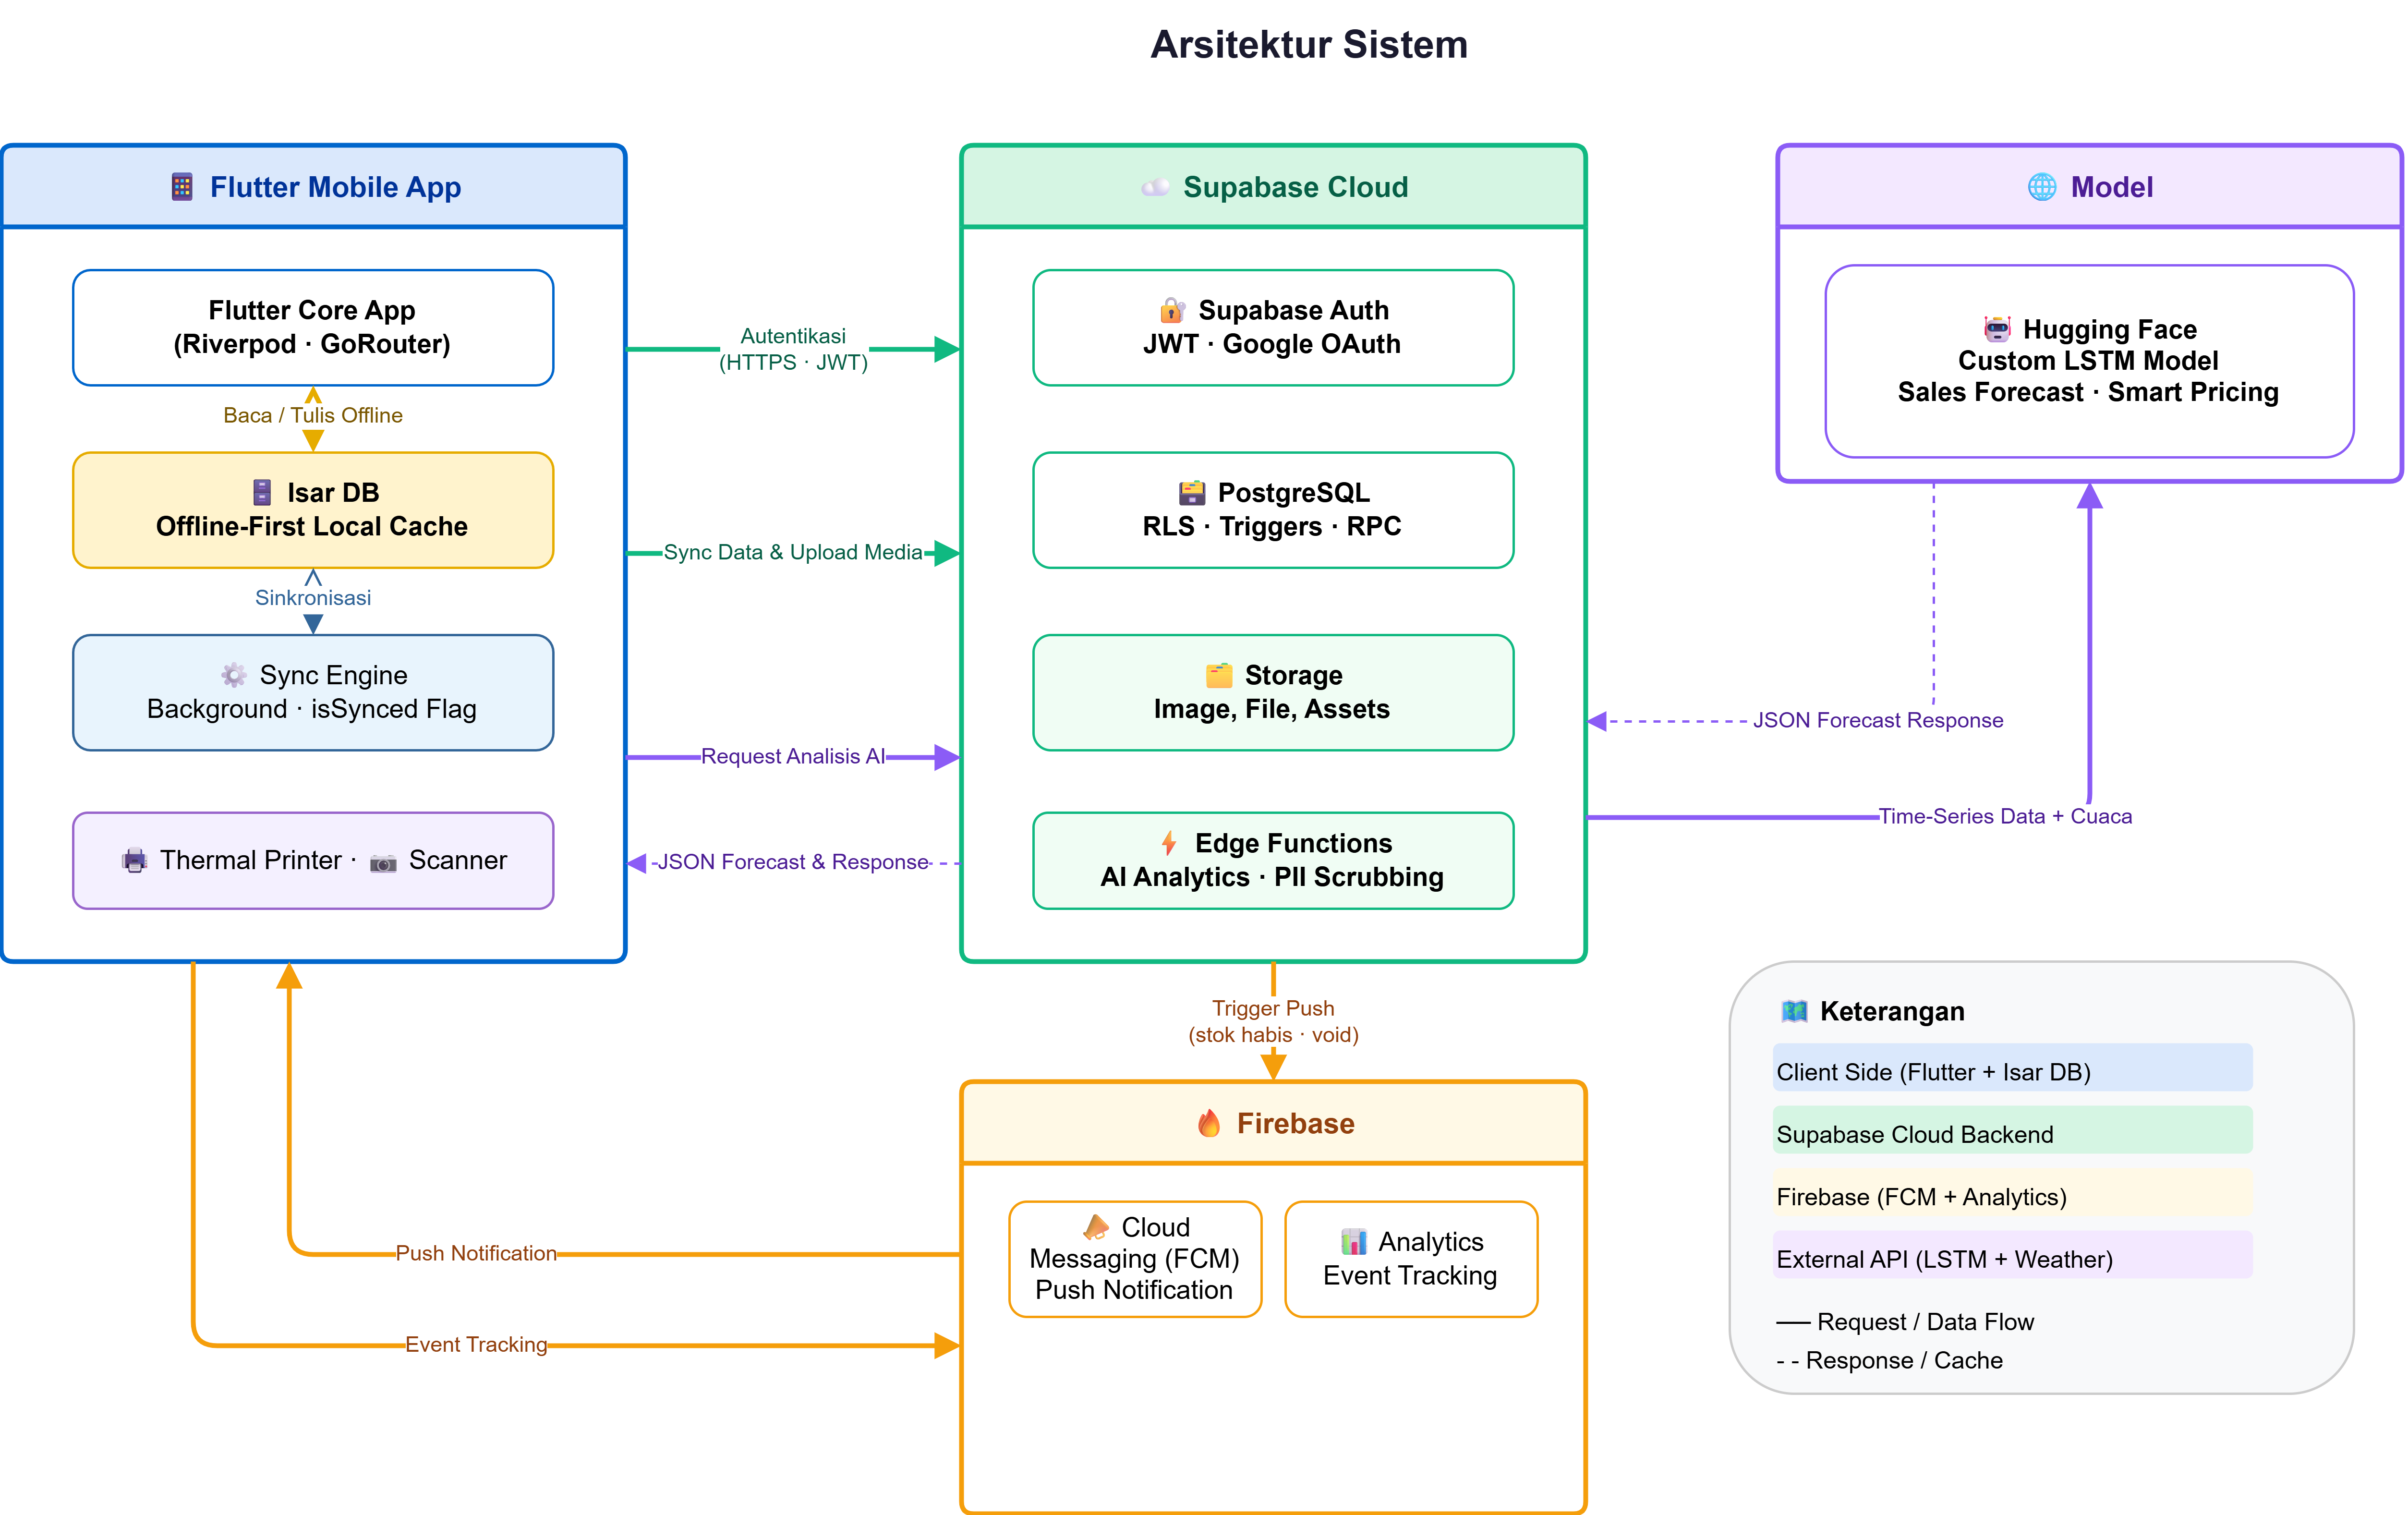
\includegraphics[width=0.88\textwidth]{arsitektur_sistem.png}}{\fbox{Arsitektur Sistem POS Offline-First}}
  \caption{Arsitektur Sistem POS Mobile Offline-First Terintegrasi Layanan Prediksi}
  \label{fig:arsitektur_sistem}
\end{figure}

\subsection{Karakteristik Dataset dan Pra-pemrosesan Data}

Dataset yang digunakan merupakan rekapitulasi transaksi penjualan harian kantin EatsTEDI UGM selama periode 26 Agustus 2024 hingga 20 Juni 2026. Agregasi penjualan dan pemfilteran hari kerja aktif menghasilkan total 313 hari transaksi aktif dengan ringkasan statistik pada Tabel \ref{tab:statistik_data}.

\begin{table}[H]
  \centering
  \caption{Statistik Ringkas Dataset Pendapatan Harian EatsTEDI UGM}
  \label{tab:statistik_data}
  \fontsize{9pt}{11pt}\selectfont
  \begin{tabular}{lc}
    \toprule
    \textbf{Karakteristik Dataset} & \textbf{Nilai Parameter} \\
    \midrule
    Jumlah hari aktif transaksi & 313 hari \\
    Rentang waktu observasi & 26 Agustus 2024 -- 20 Juni 2026 \\
    Total akumulasi omzet & Rp 471.200.494,00 \\
    Rata-rata omzet per hari aktif & Rp 1.505.433,00 \\
    Omzet tertinggi dalam satu hari & Rp 3.738.500,00 (06 Mei 2026) \\
    \bottomrule
  \end{tabular}
\end{table}

Untuk memitigasi variansi data yang ekstrem pada data deret waktu yang pendek, target prediksi tidak dimodelkan dari nilai nominal omzet mentah, melainkan dirumuskan sebagai \textit{log-return} pendapatan residual antardua hari aktif berurutan:
\begin{equation}
  y_t = \ln(1 + \text{Revenue}_t)
  \label{eq:log_revenue}
\end{equation}
\begin{equation}
  r_t = y_t - y_{t-1}
  \label{eq:log_return}
\end{equation}
dengan $r_t$ menyatakan besaran perubahan relatif omzet harian. Fitur masukan mencakup target \textit{log-return} $r_t$ beserta 6 fitur temporal yang dikodekan secara siklik menggunakan transformasi sinus-kosinus (\textit{cyclical encoding}):
\begin{equation}
  x_{\sin} = \sin\left(\frac{2\pi \cdot t}{T}\right), \quad x_{\cos} = \cos\left(\frac{2\pi \cdot t}{T}\right)
  \label{eq:cyclical}
\end{equation}
untuk variabel nomor minggu dalam setahun ($T=52$), bulan dalam setahun ($T=12$), dan hari kerja aktif dalam sepekan ($T=5$), serta 1 fitur biner penanda periode Ramadan. Variabel kuantitas dan jumlah transaksi sengaja dieliminasi dari variabel masukan guna mencegah kebocoran informasi (\textit{data leakage}). Dataset dibagi secara kronologis (tanpa pengacakan) menjadi $70\%$ data latih (219 hari), $15\%$ data validasi (46 hari), dan $15\%$ data uji (48 hari). Dengan panjang jendela pengamatan (\textit{look-back}) $L=7$ hari aktif terakhir, terbentuk 212 sekuens latih, 39 sekuens validasi, dan 41 sekuens uji dengan dimensi masukan $(N, 7, 8)$.

\subsection{Arsitektur Model LSTM dan Mekanisme Rekursif}

Arsitektur model dirancang secara efisien untuk data kecil (\textit{parsimonious}): satu lapisan LSTM dengan 24 \textit{hidden units}, lapisan \textit{Dropout} ($p=0,1$) untuk regulasi bobot, satu lapisan \textit{Dense} dengan 16 neuron beraktivasi \textit{Rectified Linear Unit} (ReLU), dan satu neuron keluaran linier untuk memprediksi $\hat{r}_t$. Struktur sel LSTM dihitung melalui persamaan gerbang \cite{hochreiter1997long}:
\begin{equation}
  f_t = \sigma(W_f \cdot [h_{t-1}, x_t] + b_f)
  \label{eq:lstm_forget}
\end{equation}
\begin{equation}
  i_t = \sigma(W_i \cdot [h_{t-1}, x_t] + b_i)
  \label{eq:lstm_input}
\end{equation}
\begin{equation}
  \tilde{C}_t = \tanh(W_c \cdot [h_{t-1}, x_t] + b_c)
  \label{eq:lstm_candidate}
\end{equation}
\begin{equation}
  C_t = f_t \odot C_{t-1} + i_t \odot \tilde{C}_t
  \label{eq:lstm_cell}
\end{equation}
\begin{equation}
  o_t = \sigma(W_o \cdot [h_{t-1}, x_t] + b_o)
  \label{eq:lstm_output}
\end{equation}
\begin{equation}
  h_t = o_t \odot \tanh(C_t)
  \label{eq:lstm_hidden}
\end{equation}

Pelatihan dilakukan menggunakan pengoptimal Adam ($\text{learning rate} = 0,001$) dengan fungsi kerugian \textit{Mean Squared Error} (MSE), \textit{batch size} 16, dan mekanisme \textit{Early Stopping} (\textit{patience} = 20) serta \textit{ReduceLROnPlateau} (\textit{patience} = 8, \textit{factor} = 0,5). Nilai nominal omzet hasil prediksi $\hat{Y}_{t}$ direkonstruksi kembali dari nilai \textit{log-return} prediksi $\hat{r}_t$ melalui:
\begin{equation}
  \hat{Y}_{t} = \exp\left( \ln(1 + Y_{t-1}) + \hat{r}_t \right) - 1
  \label{eq:inverse_log}
\end{equation}

Untuk proyeksi multi-langkah ke depan ($H=7$ hari), diterapkan mekanisme pengaman stabilisasi numerik berupa pemotongan (\textit{clipping}) pada batas persentil ke-90 data latih, faktor redaman (\textit{damping factor} $\phi=0,85^{n-1}$), serta pembatas atas historis (\textit{safety rail} $\text{REV\_CEIL}$).

\subsection{Metrik Evaluasi dan Skenario Pengujian}

Akurasi model dievaluasi menggunakan metrik \textit{Mean Absolute Error} (MAE), \textit{Root Mean Squared Error} (RMSE), dan \textit{Symmetric Mean Absolute Percentage Error} (sMAPE) \cite{hyndman2006another}:
\begin{equation}
  \text{MAE} = \frac{1}{N}\sum_{t=1}^{N} |Y_t - \hat{Y}_t|
  \label{eq:mae}
\end{equation}
\begin{equation}
  \text{RMSE} = \sqrt{\frac{1}{N}\sum_{t=1}^{N} (Y_t - \hat{Y}_t)^2}
  \label{eq:rmse}
\end{equation}
\begin{equation}
  \text{sMAPE} = \frac{100\%}{N}\sum_{t=1}^{N} \frac{2|Y_t - \hat{Y}_t|}{|Y_t| + |\hat{Y}_t|}
  \label{eq:smape}
\end{equation}
Metrik sMAPE dipilih karena memiliki batas simetris $0\%$--$200\%$ dan kebal terhadap ledakan nilai galat (\textit{exploding error}) saat omzet bernilai nol atau sangat rendah pada hari libur \cite{hyndman2006another}. Ambang kelayakan praktis yang ditetapkan untuk dapat mendukung pengambilan keputusan UMKM secara andal adalah $\text{sMAPE} < 20\%$.

Pengujian model dirancang dalam dua skenario utama:
\begin{enumerate}
  \item \textbf{Skenario 1 (Uji Akurasi Satu Langkah):} Mengukur galat MAE, RMSE, dan sMAPE model LSTM pada data uji terhadap ambang batas kelayakan praktis.
  \item \textbf{Skenario 2 (Uji Stabilitas Multi-Seed):} Melatih ulang model sebanyak 10 kali dengan \textit{random seed} berbeda ($s \in [0, 9]$) pada inisialisasi bobot NumPy, Python, dan TensorFlow guna mengukur sebaran variansi model pada volume data terbatas.
\end{enumerate}

Selain evaluasi model, sistem POS diuji fungsionalitasnya melalui metode \textit{Black Box} (12 skenario kasus penggunaan), pengujian keandalan sinkronisasi \textit{offline-first}, dan pengujian struktur logika \textit{White Box} pada jalur kritis inferensi API prediksi \cite{myers2011art, pressman2020software}.

% =========================================================================
% Section 3: Hasil dan Pembahasan
% =========================================================================
\section{Hasil dan Pembahasan}

\subsection{Implementasi Antarmuka Sistem POS dan Smart Analytics}

Aplikasi POS mobile berhasil diimplementasikan dengan antarmuka yang responsif, mencakup modul katalog produk, manajemen kategori, kasir checkout belanja, manajemen stok, dan visualisasi analisis penjualan harian. Gambar \ref{fig:smart_analytics} menampilkan antarmuka modul \textit{Smart Analytics}, di mana pemilik toko dapat memantau grafik tren omzet historis sekaligus grafik proyeksi penjualan 7 hari ke depan yang dihasilkan oleh layanan API inferensi.

\begin{figure}[H]
  \centering
  \IfFileExists{Gambar/smart_analytics.png}{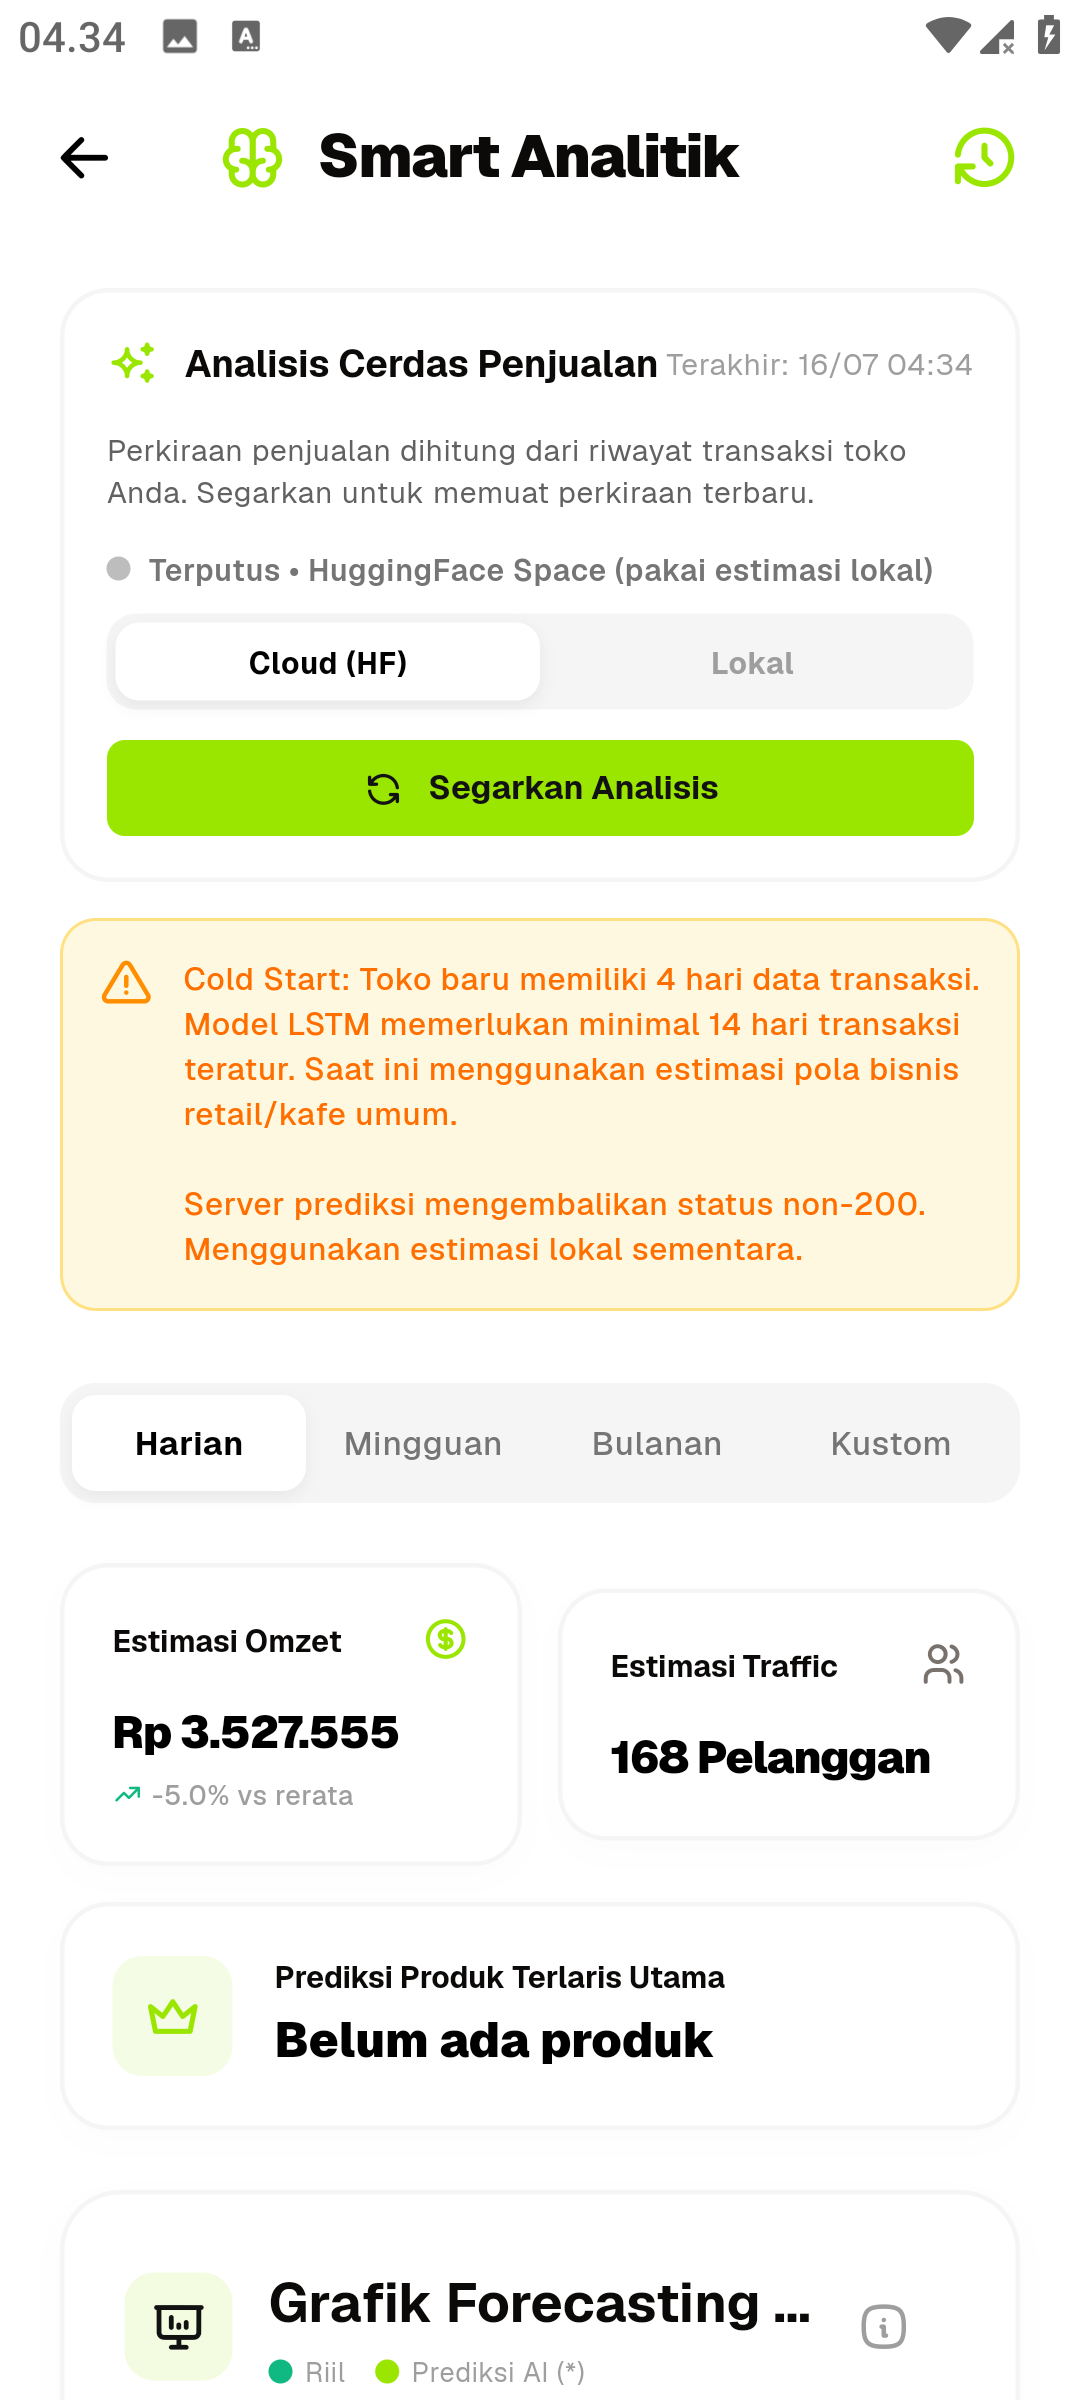
\includegraphics[width=0.42\textwidth]{smart_analytics.png}}{\fbox{Antarmuka Smart Analytics}}
  \caption{Tampilan Antarmuka Fitur Prediksi Penjualan Harian pada Aplikasi POS Mobile}
  \label{fig:smart_analytics}
\end{figure}

\subsection{Hasil Evaluasi Akurasi Model LSTM (Skenario 1)}

Hasil evaluasi performa model LSTM Hybrid pada data uji untuk skema satu langkah ke depan (\textit{one-step-ahead}) disajikan pada Tabel \ref{tab:hasil_skenario1}. Nilai yang tertera merupakan nilai rata-rata dari pengujian multi-acak.

\begin{table}[H]
  \centering
  \caption{Performa Model LSTM Hybrid pada Data Uji (One-Step-Ahead)}
  \label{tab:hasil_skenario1}
  \fontsize{9pt}{11pt}\selectfont
  \begin{tabular}{lccc}
    \toprule
    \textbf{Model Prediksi} & \textbf{MAE (Rp)} & \textbf{RMSE (Rp)} & \textbf{sMAPE (\%)} \\
    \midrule
    LSTM Hybrid (Rata-rata) & 667.718 & 897.563 & 38,06\% \\
    \bottomrule
  \end{tabular}
\end{table}

Berdasarkan Tabel \ref{tab:hasil_skenario1}, model mencatat nilai MAE Rp667.718,00 dan sMAPE sebesar 38,06\%. Nilai sMAPE ini melampaui ambang kelayakan praktis yang ditetapkan sebesar $20\%$. Gambar \ref{fig:prediksi_vs_aktual} menyajikan kurva perbandingan omzet aktual terhadap hasil prediksi LSTM Hybrid.

\begin{figure}[H]
  \centering
  \IfFileExists{Gambar/prediksi_vs_aktual.png}{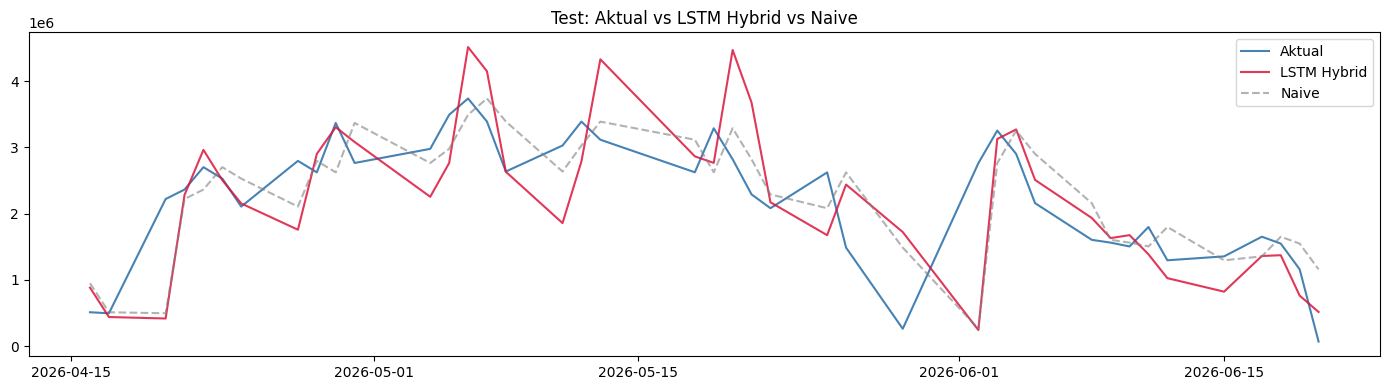
\includegraphics[width=0.88\textwidth]{prediksi_vs_aktual.png}}{\fbox{Grafik Pendapatan Aktual vs Prediksi}}
  \caption{Kurva Pendapatan Aktual terhadap Proyeksi Prediksi Model LSTM Hybrid}
  \label{fig:prediksi_vs_aktual}
\end{figure}

Visualisasi pada Gambar \ref{fig:prediksi_vs_aktual} memperlihatkan bahwa model LSTM cenderung menghasilkan pola prediksi yang terlalu halus (\textit{over-smoothing}) pada tingkat rerata deret waktu, sehingga gagal mengantisipasi lonjakan ekstrem pendapatan harian saat hari-hari sibuk perkuliahan kampus.

\subsection{Hasil Evaluasi Stabilitas Model Multi-Seed (Skenario 2)}

Hasil pengujian stabilitas model melalui pelatihan ulang 10 kali menggunakan nilai \textit{seed} acak yang berbeda dirangkum pada Tabel \ref{tab:statistik_multiseed} dan visualisasi sebaran pada Gambar \ref{fig:boxplot_multiseed}.

\begin{table}[H]
  \centering
  \caption{Statistik Performa LSTM Hybrid pada Pengujian 10 Random Seed}
  \label{tab:statistik_multiseed}
  \fontsize{9pt}{11pt}\selectfont
  \begin{tabular}{lcc}
    \toprule
    \textbf{Metrik Evaluasi} & \textbf{Rata-rata $\pm$ Simpangan Baku} & \textbf{Rentang (Min -- Maks)} \\
    \midrule
    MAE (Rp) & $667.718 \pm 145.024$ & 495.527 -- 1.048.967 \\
    RMSE (Rp) & $897.563 \pm 165.804$ & 703.721 -- 1.320.587 \\
    sMAPE & $38,06\% \pm 3,96\%$ & $29,16\% \text{ -- } 44,63\%$ \\
    \bottomrule
  \end{tabular}
\end{table}

\begin{figure}[H]
  \centering
  \IfFileExists{Gambar/boxplot_multiseed.png}{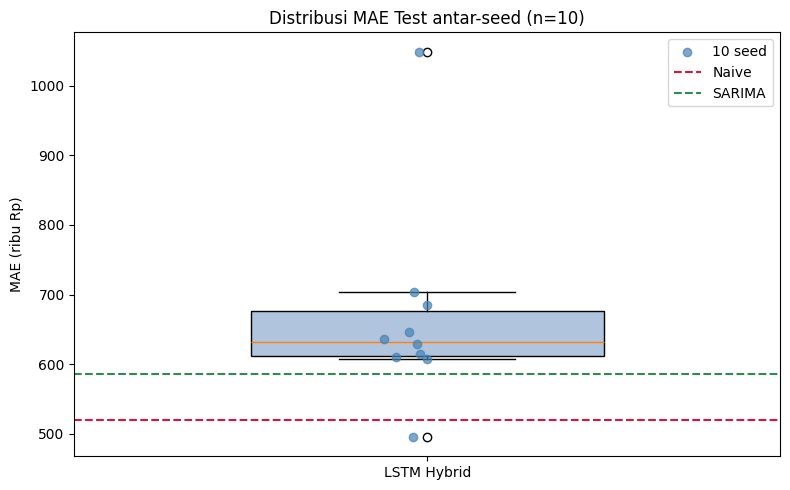
\includegraphics[width=0.68\textwidth]{boxplot_multiseed.png}}{\fbox{Boxplot Distribusi MAE Multi-Seed}}
  \caption{Distribusi Nilai MAE Hasil Pengujian Stabilitas Multi-Seed (10 Iterasi)}
  \label{fig:boxplot_multiseed}
\end{figure}

Data pada Tabel \ref{tab:statistik_multiseed} dan Gambar \ref{fig:boxplot_multiseed} menunjukkan sebaran galat yang sangat lebar: nilai MAE terburuk (Rp1.048.967,00) mencapai lebih dari dua kali lipat nilai MAE terbaik (Rp495.527,00), dengan simpangan baku mencapai Rp145.024,00. Dari 10 kali pengujian, bahkan performa terbaik sekalipada \textit{seed} ke-7 (\text{sMAPE} $29,16\%$) tetap berada di atas ambang batas praktis $20\%$. Rekapitulasi kedua skenario disajikan pada Tabel \ref{tab:rekap_skenario}.

\begin{table}[H]
  \centering
  \caption{Rekapitulasi Hasil Pengujian Kedua Skenario Model}
  \label{tab:rekap_skenario}
  \fontsize{9pt}{11pt}\selectfont
  \begin{tabularx}{\textwidth}{cXcX}
    \toprule
    \textbf{Skenario} & \textbf{Tujuan Pengujian} & \textbf{Ambang Terpenuhi?} & \textbf{Temuan Utama} \\
    \midrule
    1 & Mengukur akurasi model LSTM pada skema satu langkah & Tidak & Model mencatat sMAPE 38,06\% dan MAE Rp667.718,00, melebihi batas kelayakan praktis sMAPE $< 20\%$. \\
    \addlinespace
    2 & Menguji stabilitas model melalui 10 iterasi \textit{seed} berbeda & Tidak & Sebaran MAE sangat lebar (Rp495.527 -- Rp1.048.967). Model sangat sensitif terhadap inisialisasi bobot acak. \\
    \bottomrule
  \end{tabularx}
\end{table}

\subsection{Hasil Pengujian Sistem (Black Box, Sinkronisasi, dan White Box)}

Pengujian fungsionalitas sistem menggunakan metode \textit{Black Box} mencakup 12 kasus penggunaan utama, sebagaimana disajikan pada Tabel \ref{tab:blackbox}. Seluruh fungsionalitas berhasil memenuhi kriteria yang diharapkan ($100\%$ sukses).

\begin{table}[H]
  \centering
  \caption{Hasil Pengujian Fungsionalitas Sistem (Black Box Testing)}
  \label{tab:blackbox}
  \fontsize{9pt}{11pt}\selectfont
  \begin{tabularx}{\textwidth}{clXc}
    \toprule
    \textbf{No} & \textbf{Fitur / Skenario Pengujian} & \textbf{Hasil yang Diharapkan} & \textbf{Status} \\
    \midrule
    1 & Registrasi Toko Baru & Akun owner dan profil toko tersimpan di basis data awan & Berhasil \\
    2 & Autentikasi Login Pengguna & Masuk ke dasbor utama sesuai hak akses peran (Owner/Kasir) & Berhasil \\
    3 & Checkout Transaksi Belanja & Transaksi tercatat, stok barang berkurang otomatis di lokal & Berhasil \\
    4 & Manajemen Katalog Produk & Tambah, ubah, dan hapus data produk di katalog & Berhasil \\
    5 & Manajemen Kategori Menu & Mengelompokkan item produk berdasarkan kategori menu & Berhasil \\
    6 & Audit Riwayat Mutasi Stok & Pencatatan penambahan dan pengurangan stok pada log mutasi & Berhasil \\
    7 & Dasbor Ringkasan Bisnis & Menampilkan total omzet dan grafik ringkasan transaksi & Berhasil \\
    8 & Prediksi Smart Analytics & Grafik proyeksi penjualan 7 hari tampil pada antarmuka & Berhasil \\
    9 & Siaran Notifikasi Kasir & Pengiriman pesan notifikasi dari owner diterima oleh kasir & Berhasil \\
    10 & Sinkronisasi Data Transaksi & Transaksi lokal terunggah otomatis saat jaringan pulih & Berhasil \\
    11 & Manajemen Akun Staf & Owner berhasil menambah dan mengatur kredensial staf kasir & Berhasil \\
    12 & Pengaturan Informasi Toko & Perubahan profil identitas toko tersimpan dengan benar & Berhasil \\
    \bottomrule
  \end{tabularx}
\end{table}

Hasil pengujian mekanisme sinkronisasi \textit{offline-first} pada Tabel \ref{tab:sinkronisasi} membuktikan bahwa transaksi tetap dapat dilakukan saat perangkat kasir berada dalam kondisi luring (\textit{offline}), dan data berhasil diunggah secara konsisten ke Supabase tanpa kehilangan atau duplikasi data saat koneksi kembali aktif.

\begin{table}[H]
  \centering
  \caption{Hasil Pengujian Mekanisme Sinkronisasi Offline-First}
  \label{tab:sinkronisasi}
  \fontsize{9pt}{11pt}\selectfont
  \begin{tabularx}{\textwidth}{clXc}
    \toprule
    \textbf{No} & \textbf{Skenario Pengujian} & \textbf{Hasil Pengujian Aktual} & \textbf{Status} \\
    \midrule
    1 & Checkout kasir saat kondisi luring & Transaksi tersimpan di Isar DB lokal (\texttt{is\_synced = false}), stok berkurang di lokal & Berhasil \\
    2 & Buka riwayat kasir saat luring & Daftar transaksi lokal tampil instan tanpa galat sambungan & Berhasil \\
    3 & Reaktivasi koneksi internet (daring) & \textit{SyncEngine} mendeteksi jaringan dan mengunggah data lokal ke Supabase & Berhasil \\
    4 & Verifikasi data di basis data awan & Data transaksi masuk ke Supabase, status lokal berubah (\texttt{is\_synced = true}) & Berhasil \\
    \bottomrule
  \end{tabularx}
\end{table}

Pengujian \textit{White Box} dengan teknik \textit{basis path testing} diterapkan pada 7 jalur logika kritis di fungsi peramalan API (\texttt{by\_dow}, penanganan \texttt{smape}, dan stabilisasi \texttt{forecast\_hybrid\_stable}), seperti terangkum pada Tabel \ref{tab:whitebox}. Seluruh jalur penanganan berjalan sesuai rancangan logika.

\begin{table}[H]
  \centering
  \caption{Hasil Pengujian White Box pada Fungsi Kritis Layanan Prediksi}
  \label{tab:whitebox}
  \fontsize{9pt}{11pt}\selectfont
  \begin{tabularx}{\textwidth}{cllXc}
    \toprule
    \textbf{No} & \textbf{Fungsi Logika} & \textbf{Kondisi Masukan} & \textbf{Hasil yang Diharapkan} & \textbf{Status} \\
    \midrule
    1 & \texttt{by\_dow} & Riwayat hari kerja $\ge k$ & Rata-rata dari $k$ kemunculan terakhir hari kerja & Berhasil \\
    2 & \texttt{by\_dow} & Riwayat hari kerja $< k$ & Rata-rata dari seluruh kemunculan hari kerja yang ada & Berhasil \\
    3 & \texttt{by\_dow} & Riwayat hari kerja tidak ada & \textit{Fallback} menggunakan rata-rata 10 hari aktif terakhir & Berhasil \\
    4 & \texttt{smape} & Nilai aktual dan prediksi bernilai 0 & Menghasilkan galat 0 tanpa \textit{division by zero} & Berhasil \\
    5 & \texttt{forecast\_stable} & \textit{Log-return} melampaui persentil 90 & Nilai dipotong tepat pada batas persentil 90 (\textit{clipping}) & Berhasil \\
    6 & \texttt{forecast\_stable} & Langkah peramalan ke-$n$ ($n>1$) & Perubahan teredam faktor pengali $\phi^{n-1}$ (\textit{damping}) & Berhasil \\
    7 & \texttt{forecast\_stable} & Omzet melampaui omzet puncak & Nilai dibatasi tepat pada batas atas (\textit{safety rail}) & Berhasil \\
    \bottomrule
  \end{tabularx}
\end{table}

\subsection{Pembahasan dan Posisi Temuan terhadap Penelitian Terdahulu}

Hasil pengujian akurasi dan stabilitas model mengungkapkan fakta empiris yang penting mengenai penerapan model \textit{deep learning} pada skala UMKM:
\begin{enumerate}
  \item \textbf{Akar Keterbatasan Performa:} Tingginya nilai sMAPE ($38,06\%$) dan lebarnya dispersi nilai MAE bukan disebabkan oleh kesalahan sintaksis arsitektur model, melainkan bersumber dari keterbatasan intrinsik volume dataset (hanya 313 hari aktif) yang menyusut menjadi 212 sekuens latih. Dalam ranah \textit{deep learning}, jumlah sampel ini tergolong sangat kecil untuk melatih bobot jaringan secara konvergen.
  \item \textbf{Karakteristik Data Kampus yang Terputus-putus:} Kalender akademik menimbulkan banyak hari libur (semesteran pada Januari dan Juli) serta akhir pekan. Pemfilteran hari aktif ($\text{revenue} > 0$) menghasilkan jeda hari kalender (\textit{gap days}) yang tidak seragam (dapat mencapai lebih dari 10 hari). Hal ini melanggar asumsi deret waktu reguler yang disyaratkan oleh LSTM.
  \item \textbf{Transparansi Metodologis:} Berbeda dengan penelitian sebelumnya yang kerap melaporkan akurasi satu kali latih (\textit{single-run}) yang kebetulan optimal, temuan ini secara terbuka menunjukkan batas bawah kelayakan data. Pada volume data di bawah dua tahun, pendekatan heuristik seperti \textit{Seasonal-Naive} lebih stabil secara operasional. Model LSTM baru direkomendasikan untuk dievaluasi kembali setelah riwayat transaksi UMKM terakumulasi minimal 3 hingga 5 tahun operasional penuh.
  \item \textbf{Keunggulan Arsitektur Sistem POS:} Keterbatasan model prediksi tidak mengganggu kinerja operasional kasir harian karena arsitektur sistem memisahkan fungsi POS luring dengan modul analitik berbasis API (\textit{model-agnostic}).
\end{enumerate}

% =========================================================================
% Section 4: Kesimpulan
% =========================================================================
\section{Kesimpulan}

Berdasarkan perancangan, implementasi, dan pengujian yang telah dilakukan, dapat disimpulkan bahwa:
\begin{enumerate}
  \item Aplikasi \textit{Point of Sale} berbasis \textit{mobile} dengan arsitektur \textit{offline-first} (Flutter, Isar DB, Supabase, dan Flask API) berhasil dibangun dan terintegrasi penuh. Pengujian \textit{black box} pada 12 kasus penggunaan, pengujian mekanisme sinkronisasi data lokal-awan, serta pengujian \textit{white box} pada fungsi inferensi seluruhnya berhasil dengan tingkat keberhasilan $100\%$, menjamin keandalan transaksi kasir tanpa ketergantungan jaringan internet.
  \item Penerapan model LSTM pada dataset riil transaksi EatsTEDI UGM (313 hari aktif) menghasilkan evaluasi rata-rata MAE Rp667.718,00 dan sMAPE 38,06\% pada skema satu langkah ke depan, melampaui ambang kelayakan praktis operasional yang ditetapkan ($\text{sMAPE} < 20\%$).
  \item Pengujian kestabilan \textit{multi-seed} mengungkap dispersi galat yang lebar (MAE Rp495.527,00 hingga Rp1.048.967,00), membuktikan bahwa model \textit{deep learning} sangat peka terhadap inisialisasi bobot awal pada volume data latih yang kecil. Penelitian ini menyimpulkan bahwa metode \textit{deep learning} belum layak secara praktis diterapkan pada data UMKM dengan riwayat kurang dari dua tahun, dan merekomendasikan evaluasi ulang setelah data mencapai 3--5 tahun operasional atau dengan penambahan variabel interval hari kalender (\textit{gap days}).
\end{enumerate}


% =========================================================================
% References (IEEE Style)
% =========================================================================
\begin{thebibliography}{99}
\fontsize{8pt}{9.8pt}\selectfont
\setlength{\itemsep}{0.5pt}
\setlength{\parskip}{0pt}

\bibitem{mansur2025sales}
S. Mansur, K. Sattar, S. E. Hosseini, S. Pervez, I. Ahmad, K. Saleem, and A. Z. Elhendi, ``Sales Forecasting for Retail Stores Using Hybrid Neural Networks and Sales-Affecting Variables,'' \textit{PeerJ Computer Science}, vol. 11, Art. no. e3058, 2025, doi: 10.7717/peerj-cs.3058.

\bibitem{hochreiter1997long}
S. Hochreiter and J. Schmidhuber, ``Long Short-Term Memory,'' \textit{Neural Computation}, vol. 9, no. 8, pp. 1735--1780, 1997, doi: 10.1162/neco.1997.9.8.1735.

\bibitem{mitra2024harnessing}
M. Mitra, S. Roy, S. De, S. Bhattacharyya, J. Platos, and V. Snasel, ``Harnessing LSTM Neural Networks and Hyperparameter Optimization for Precise Sales Forecasting in Retail,'' in \textit{Proc. 10th Int. Conf. Advanced Intelligent Systems and Informatics (AISI 2024)}, Cham, Switzerland: Springer, 2024, pp. 120--132, doi: 10.1007/978-3-031-71619-5\_11.

\bibitem{moraes2024hybrid}
T. de Castro Moraes, X.-M. Yuan, and E. P. Chew, ``Hybrid Convolutional Long Short-Term Memory Models for Sales Forecasting in Retail,'' \textit{Journal of Forecasting}, vol. 43, no. 5, pp. 1278--1293, 2024, doi: 10.1002/for.3073.

\bibitem{makridakis2022m5}
S. Makridakis, E. Spiliotis, and V. Assimakopoulos, ``The M5 Competition: Background, Organization, and Implementation,'' \textit{International Journal of Forecasting}, vol. 38, no. 4, pp. 1325--1336, 2022, doi: 10.1016/j.ijforecast.2021.07.007.

\bibitem{yadav2025retail}
P. Yadav and C. R. Barde, ``Retail Real-Time Sales Prediction System Using LSTM and XGBoost,'' \textit{International Journal of Advanced Research in Computer and Communication Engineering (IJARCCE)}, vol. 14, no. 4, pp. 45--52, 2025.

\bibitem{sembiring2025analisa}
R. A. Sembiring and Y. Sary, ``Analisa dan Implementasi Long Short-Term Memory (LSTM) dalam Kebutuhan Persediaan Barang di PT. Gunung Sari Indonesia,'' \textit{Jurnal Ilmiah Teknik Mesin, Elektro dan Komputer}, vol. 5, no. 1, pp. 12--21, 2025.

\bibitem{jannah2025analisis}
U. M. Jannah, A. S. Wiguna, dan D. P. Hapsari, ``Analisis Prediksi Penjualan Isi Ulang Air Galon Menggunakan Metode LSTM dan SARIMA,'' \textit{Jurnal Teknologi Informasi dan Multimedia}, vol. 7, no. 1, pp. 33--42, 2025.

\bibitem{verdiyanto2025pengembangan}
R. Verdiyanto, D. Hartanti, and E. Purwanto, ``Pengembangan Aplikasi Point of Sales untuk Prediksi Penjualan Harian Usaha Minuman Menggunakan Algoritma Random Forest Regression,'' \textit{Infotek: Jurnal Informatika dan Teknologi}, vol. 8, no. 2, pp. 110--120, 2025.

\bibitem{sipayung2020evaluasi}
E. M. Sipayung, C. Fiarni, and Wawan, ``Evaluasi Penggunaan Aplikasi Point of Sale Menggunakan Technology Acceptance Model pada UMKM,'' \textit{Jurnal Nasional Teknik Elektro dan Teknologi Informasi (JNTETI)}, vol. 9, no. 1, pp. 18--24, 2020, doi: 10.22146/jnteti.v9i1.116.

\bibitem{siddik2020rancang}
M. Siddik and S. Samsir, ``Rancang Bangun Sistem Informasi POS (Point of Sale) untuk Kasir Menggunakan Konsep Bahasa Pemrograman Orientasi Objek,'' \textit{JOISIE (Journal of Information Systems and Informatics Engineering)}, vol. 4, no. 1, pp. 43--48, 2020, doi: 10.35145/joisie.v4i1.607.

\bibitem{hyndman2021forecasting}
R. J. Hyndman and G. Athanasopoulos, \textit{Forecasting: Principles and Practice}, 3rd ed. Melbourne, Australia: OTexts, 2021.

\bibitem{box2015time}
G. E. P. Box, G. M. Jenkins, G. C. Reinsel, and G. M. Ljung, \textit{Time Series Analysis: Forecasting and Control}, 5th ed. Hoboken, NJ, USA: John Wiley \& Sons, 2015.

\bibitem{hyndman2006another}
R. J. Hyndman and A. B. Koehler, ``Another Look at Measures of Forecast Accuracy,'' \textit{International Journal of Forecasting}, vol. 22, no. 4, pp. 679--688, 2006, doi: 10.1016/j.ijforecast.2006.03.001.

\bibitem{flutter2026docs}
Google LLC, ``Flutter Documentation,'' 2026. [Online]. Available: \url{https://docs.flutter.dev/}. [Accessed: 29-Jul-2026].

\bibitem{pressman2020software}
R. S. Pressman and B. R. Maxim, \textit{Software Engineering: A Practitioner's Approach}, 9th ed. New York, NY, USA: McGraw-Hill Education, 2020.

\bibitem{myers2011art}
G. J. Myers, C. Sandler, and T. Badgett, \textit{The Art of Software Testing}, 3rd ed. Hoboken, NJ, USA: John Wiley \& Sons, 2011.

\bibitem{iso29119}
\textit{Software and Systems Engineering --- Software Testing --- Part 4: Test Techniques}, ISO/IEC/IEEE Standard 29119-4:2021, 2021.

\bibitem{sigala2019big}
M. Sigala, A. Beer, L. Hodgson, and A. O'Connor, \textit{Big Data for Measuring the Impact of Tourism Economic Development Programmes: A Process and Quality Criteria Framework for Using Big Data}. Adelaide, Australia: Centre for Tourism and Leisure Management, 2019.

\bibitem{nguyen2019machine}
G. Nguyen \textit{et al.}, ``Machine Learning and Deep Learning frameworks and libraries for large-scale data mining: a survey,'' \textit{Artif. Intell. Rev.}, vol. 52, no. 1, pp. 77--124, 2019, doi: 10.1007/s10462-018-09679-z.

\bibitem{vinayakumar2019deep}
R. Vinayakumar, M. Alazab, K. P. Soman, P. Poornachandran, A. Al-Nemrat, and S. Venkatraman, ``Deep Learning Approach for Intelligent Intrusion Detection System,'' \textit{IEEE Access}, vol. 7, pp. 41525--41550, 2019, doi: 10.1109/ACCESS.2019.2895334.

\bibitem{ang2019deployment}
L. M. Ang, K. P. Seng, G. K. Ijemaru, and A. M. Zungeru, ``Deployment of IoV for Smart Cities: Applications, Architecture, and Challenges,'' \textit{IEEE Access}, vol. 7, pp. 6473--6492, 2019, doi: 10.1109/ACCESS.2018.2887076.

\bibitem{lau2019survey}
B. P. L. Lau \textit{et al.}, ``A survey of data fusion in smart city applications,'' \textit{Inf. Fusion}, vol. 52, pp. 357--374, 2019, doi: 10.1016/j.inffus.2019.05.004.

\bibitem{wu2019large}
Y. Wu \textit{et al.}, ``Large scale incremental learning,'' in \textit{Proc. IEEE Comput. Soc. Conf. Comput. Vis. Pattern Recognit. (CVPR)}, 2019, pp. 374--382, doi: 10.1109/CVPR.2019.00046.

\bibitem{mosavi2019prediction}
A. Mosavi, S. Shamshirband, E. Salwana, K. wing Chau, and J. H. M. Tah, ``Prediction of multi-inputs bubble column reactor using a novel hybrid model of computational fluid dynamics and machine learning,'' \textit{Eng. Appl. Comput. Fluid Mech.}, vol. 13, no. 1, pp. 482--492, 2019, doi: 10.1080/19942060.2019.1613448.

\bibitem{sadowski2019data}
J. Sadowski, ``When data is capital: Datafication, accumulation, and extraction,'' \textit{Big Data Soc.}, vol. 6, no. 1, pp. 1--12, 2019, doi: 10.1177/2053951718820549.

\end{thebibliography}

\end{document}
